% coding:utf-8

%----------------------------------------
%FOSAMATH, a LaTeX-Code for a mathematical summary for basic analysis
%Copyright (C) 2013, Daniel Winz, Ervin Mazlagic, Adrian Imboden, Philipp Langer

%This program is free software; you can redistribute it and/or
%modify it under the terms of the GNU General Public License
%as published by the Free Software Foundation; either version 2
%of the License, or (at your option) any later version.

%This program is distributed in the hope that it will be useful,
%but WITHOUT ANY WARRANTY; without even the implied warranty of
%MERCHANTABILITY or FITNESS FOR A PARTICULAR PURPOSE.  See the
%GNU General Public License for more details.
%----------------------------------------

% coding:utf-8
\section{Umwandlung Stern $\leftrightarrow$ Dreieck}
\begin{figure}[h!]
\centering
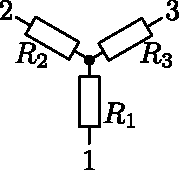
\includegraphics[scale=\schscale]{star_sch.pdf}

\vspace{5mm}

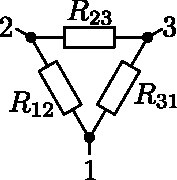
\includegraphics[scale=\schscale]{tri_sch.pdf}
\label{sch:tristar}
\caption{Srern- und Dreieckschaltung}
\end{figure}

\subsection{Umwandlung Dreieck $\to$ Stern}
\[ \begin{matrix}
R_1 = \dfrac{R_{12} \cdot R_{31}}{R_{12} + R_{23} + R_{31}}\\\\
R_2 = \dfrac{R_{23} \cdot R_{12}}{R_{12} + R_{23} + R_{31}}\\\\
R_3 = \dfrac{R_{31} \cdot R_{23}}{R_{12} + R_{23} + R_{31}}\\\\
\end{matrix} \]

\subsection{Umwandlung Stern $\to$ Dreieck}
\[ \begin{matrix}
R_{12} = \dfrac{R_1 \cdot R_2 + R_2 \cdot R_3 + R_3 \cdot R_1}{R_3}\\\\
R_{23} = \dfrac{R_1 \cdot R_2 + R_2 \cdot R_3 + R_3 \cdot R_1}{R_1}\\\\
R_{31} = \dfrac{R_1 \cdot R_2 + R_2 \cdot R_3 + R_3 \cdot R_1}{R_2}\\\\
\end{matrix} \]